\section{Evaluation}
\label{sec:evaluation}
In order to evaluate the efficacy of our approach, we evaluated \sysname in three phases:

In the \textbf{first phase} (\secref{sec:normal_operation}, we ran experiments on multiple doorways, with different characteristics---like light levels, flooring, doorway heights and doorway widths.
For each experiment, we primarily evaluated \sysname's ability to detect someone passing through and determine the person's direction of movement.
In this phase, we also tested the systems robustness to human variations, such as height, clothing, and hair color by considering a diverse group of subjects.
Our study was conducted on \numDoors different doorways with \numPeople different people for a total of \numExp different doorway events (each person walked through multiple times per doorway).\footnote{This study was approved by our Institutional Review Board.}

In the \textbf{second phase} (\secref{sec:confounding}), we tried to push the limits of the device, examining the factors that affect its accuracy, performance and availability.
These factors included the effect of adverse lighting conditions, walking speed and shorter delays between doorway events.
We also investigated other events that might get falsely detected as doorway events.

In the \textbf{third phase} (\secref{sec:microbenchmarks}) we explore the energy harvesting ability and gather microbenchmarks of the energy consumption of the parts of the \sysname system.

\begin{table*}[t]
\footnotesize
	\begin{tabular}{@{}p{0.6in}p{0.5in}p{0.5in}p{0.45in}p{0.6in}p{0.3in}p{0.7in}p{0.7in}p{0.5in}@{}}
	\toprule
	\multirow{2}{*}{\textbf{Doorway \#}}	&	\multicolumn{2}{c}{\textbf{Light Intensity (lux)}} & \multicolumn{2}{c}{\textbf{Flooring}} & \multicolumn{1}{c}{\textbf{Enough}} & \multicolumn{1}{c}{\textbf{Total}} & \multicolumn{1}{c}{\textbf{Detection}} & \multicolumn{1}{c}{\textbf{Direction}} 		\\
	& Inside & Outside & Inside & Outside & \multicolumn{1}{c}{\textbf{Light?}} & \multicolumn{1}{c}{\textbf{Events \#}} & \multicolumn{1}{c}{\textbf{Accuracy(\%)}} & \multicolumn{1}{c}{\textbf{Accuracy(\%)}}\\\midrule
	1 & 86 & 96\textsuperscript{*} & Tile & Tile & Yes & 162 & 93.82 & 98.02 \\ %Lab Door
	2 & 86\textsuperscript{*} & 64 & Carpet & Tile & Yes & 63 & 90.48 & 78.94 \\ %224
	3 & 71 & 55 & Carpet & Tile & Yes & 106 & 100 & 98.11 \\	%Jacob's office
	4 & 96 & 111\textsuperscript{*} & Tile & Tile & Yes & 106 & 100 & 98.11 \\ %232
	5 & 55 & 55 & Tile & Tile & Yes & 112 & 99.1 & 94.59 \\ %hallway1
	6 & 55 & 71 & Tile & Tile & Yes & 102 & 100 & 96.08 \\\midrule %hallway2
	7 & 40 & 71 & Carpet & Tile & No & - & - & - \\ %226-1
	8 & 24 & 72 & Carpet & Tile & No & - & - & - \\ %226-2
	9 & 24 & 55 & Tile & Tile & No & - & - & - \\ %hallway-119
	\bottomrule
	\end{tabular}
	\caption{Evaluation results with 12 test subjects having variable heights, hair color, and clothing as described in \secref{sec:normal_operation}. We tested 9 different doorways, from which 6 had enough light to power \sysname. We ran multiple people through each of these 6 doorways, noting the detection accuracy and how many of the detected events had correct direction. These results show that an adequately-lit \sysname occupancy monitor can accurately detect doorway events and their directions.
	\vspace{1mm}
	\\\textsuperscript{*}Mixed Lighting --- Combined natural and artificial light
	\label{tab:detection}}

\end{table*}



\subsection{Methodology and Claims}
The following experiments attempt to address the goals defined in \secref{sec:system}.
We address system availability~(Goal~1) by demonstrating the low power draw of the system itself and the number of times it caught doorway events (and the number of doorway events missed) for each doorway test.
% the minimum light intensity at which \sysname can sustain operation and detect doorway events.
Further, we evaluated the accuracy in determining the direction~(Goal~2) by observing how often \sysname correctly determined walking direction.
We explored variable lighting conditions~(Goal~3) by testing the device under \numDoors different doorways with diverse lighting conditions, both typical and adverse.
We address human variation~(Goal~4) by evaluating different walking speeds and the effect of clothing and hair color/hair covering on detection patterns.
We claim that~(Goal~5), concerning form factor, is addressed by our prototype and slim mechanical design, described in \secref{sec:implementation}.

We also have attempted to test the limits of the device, by varying different factors to see when the device stops working and generating conditions that can confound the sensor.
We acknowledge that these experiments are best effort, and cannot hope to cover all variability and confounding factors of tracking of diverse persons and buildings, but they do give a broad sense of the capabilities and limitations of \sysname.

To process and enable data collection in our experiments, we gather all electrical signal measurements, except where specified otherwise, using the Saleae Logic~16 logic analyzer\footnote{https://www.saleae.com}, at a sampling rate of 5KS/s.
The analyzer has high impedance ADC's allowing for unobtrusive monitoring of all signals.
This sampling rate is sufficient to detect events on the doorway as we are monitoring fairly slow-varying events.
We manually recorded the direction of each doorway event as ground truth to verify the accuracy of \sysname in event detection, then compared the ground truth results with the results measured by the logic analyzer.
The light intensity levels were measured using the TSL2561 Light-to-digital converter from Texas Advanced Optoelectronic Solutions.\footnote{https://cdn-shop.adafruit.com/datasheets/TSL2561.pdf}
These converters were aligned to the same angle as the solar panels in both directions to get accurate light intensities falling on the panels.

Finally, we note that it is difficult to fairly compare the performance of different occupancy-monitoring systems except in their accuracy. For example, CeilingSee~\cite{yang2017ceilingsee} uses 16 devices to instrument a room, while \sysname and SonicDoor~\cite{sonicdoor-buildsys2017} place one device in the doorway, and AURES~\cite{shih2016aures} places a single device in the middle of a room. 
For this reason, we investigate the accuracy of \sysname against our manually gathered ground truth (visually verifying a person entering or exiting the room) instead of comparing to another occupancy-detection system.

%%only if time allows:
%%%passing vs. normal entering and exiting of the room
%%%what multiple people entering in close succession looks like to the system and can the system tell the difference between the systems.

%Notes on current testing plan environment:
%tile floor, semi reflective
%door open
%lights on on both sides of the door
%16 solar panels that are alternatively tilted by 10 degrees in either direction (8 panels on each side)
%walking at normal speed through the center of the doorway

%In order to test how well \sysname fares in terms of the availability goal, we tried turning down the light levels till \sysname stopped sustaining operation. Our aim in performing this experiment is to find a threshold above which \sysname sustains operation and is available for detecting ephemeral doorway events as they occur.
%We found that \sysname stops sustaining operation below XXYYZZ lux. This is an acceptable threshold as the average light levels in office environments will be greater than or equal to \SI{70}{\lux}. Even when the light levels fall significantly lower till \SI{40}{\lux}, we are able to detect events but it does affect our direction detection, as outlined in the next section.


\subsection{Normal Operation}
\label{sec:normal_operation}

\noindpar{Experiment Goals:}
This section presents a thorough testing of the \sysname sensor across multiple different doorways with a diverse group of subjects.
The goal of this evaluation is to understand how well \sysname can perform occupancy monitoring.
The definition of occupancy monitoring in this context is detecting doorway events caused by people walking \textit{under} the doorway, and further detecting the direction of their movement.

\noindpar{Experiment Overview:}
We ran the experiment with twelve~(12) different participants, with different physical characteristics---heights ranging from 5'4'' to 6'4'' and hair color ranging from blond to brown and black.
Our test group included a wide range of clothing colors (light and dark) and a variety of head coverings.


For this experiment, we affixed the \sysname prototype to the top of \numDoors different doorways.
We have summarized each doorway in \tabref{tab:detection}, outlining details such as the light intensity levels on both sides, type of flooring, etc.
For each doorway, we maintained test subject diversity, in order to characterize \sysname's performance, independent of the characteristics of individual subjects.
For doorways with doors, the door remained open all through the experiments.
%This was done since
Each participant walked in and out of the room five times in each direction.

\noindpar{Results:}
The results of this experiment are shown in \tabref{tab:detection}, where we tested the system on a total of 651 individual events.
Each \textit{event} consists of one person walking through one doorway one time.
\sysname was successful in detecting doorway events and also the direction people were traveling through the doorway.
It detected a total of \numDet events out of \numExp, giving an overall detection accuracy of \SysAccuracy.
Furthermore, it determined the walking direction correctly for a total of \numDir events, which is \dirAccuracy of the total events detected.
\sysname's performance was consistent across all test subjects, independent of human variations like height, hair color, and clothing.



\subsection{Factors affecting \sysname's operation}
\label{sec:confounding}

\noindpar{Experiment Goals:}
The effectiveness of \sysname in occupancy monitoring is demonstrated through the experiments outlined in \secref{sec:normal_operation}.
In this section, we examine factors that affect \sysname's performance as an occupancy-monitoring sensor.
It would be impossible to exhaustively study all possible combinations of every factor.
Instead, in this section we explore how \sysname reacts to a variety of conditions and behaviors that it will encounter in actual deployments.


\noind{We explored the following factors:}
\subsubsection{Light intensity:}
We tested the availability of \sysname on different doorways and have reported our findings in \tabref{tab:detection}.
The solar panels powering \sysname are sensitive to light in the visible as well as the IR spectrum.
As a result, to provide a more complete analysis of the illumination around a doorway, we could not rely simply on a lux meter, which only provides information about visible light.
We used a TSL2561 sensor that measures both mixed signal (visible and IR) data along with purely IR data, and outputs the combined illumination value in lux.
After analysing the data in \tabref{tab:detection}, we can see that our current prototype is fully functional on doorways with light levels above at least 55~lux on both sides.
An average room/hallway in an office-style setting has light levels around 70~lux, which is sufficient to power the \sysname sensor.
It is worth noting that we can customize \sysname for exceptionally dark doorways either by increasing the number of solar panels without changing the working of the system itself, or by employing input booster circuits like the ones used in CleanCut~\cite{colin2018cleancut}.

\subsubsection{Walking Speed:}
\sysname detects people walking under doorways based on the changes they cause in the amount of energy harvested.
This means that there exists a theoretical limit to how slowly someone can walk through before their movement becomes imperceptible to the system.
In order to evaluate this limit, we asked test subjects to walk under the sensor at different speeds.
We used a metronome to which the subjects could match their steps in order to achieve a consistent even speed.
With extremely slow walking (slower than 1~ft/s), we did observe decreased accuracies.
\sysname occasionally detected a slow-moving doorway event as two events.
No test subjects have yet been able to walk slowly enough to avoid detection entirely.
We don't consider this to be a problem for \sysname, since in practice, people don't often move at such slow speeds.

\subsubsection{Door Width and Height:}
All doors except door \#4 (in \tabref{tab:detection}) were 80 inches tall, door \#4 was 87 inches tall. 
All doors except door \#6 were 34.5 inches wide, while \#6 was 58.5 inches wide.
A typical interior doorway is 32 inches by 80 inches.
In our experiments, the door width and height had no significant effect on the accuracy, however, we only tested when a single person went through a wide door, and we did not control for participants walking through the middle or side of the door (they were asked to walk naturally).


\begin{figure*}[t]
    \centering
    \begin{subfigure}[b]{0.45\textwidth}
        \centering
        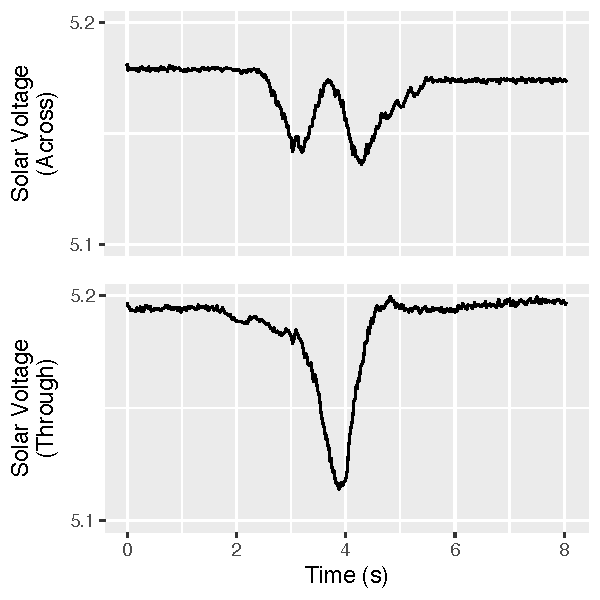
\includegraphics[width=\columnwidth]{figs/spotlight.pdf}
        \caption{These traces show the solar panel output in the presence of the ``Spotlight'' effect. The top figure shows the response when someone walks \textit{across} the ``Spotlight'', while the bottom one shows the response when someone walks \textit{through} the door.}
        \label{fig:spotlight}
    \end{subfigure}%
    %
    \hspace{10pt}
    \begin{subfigure}[b]{0.45\textwidth}
        \centering
        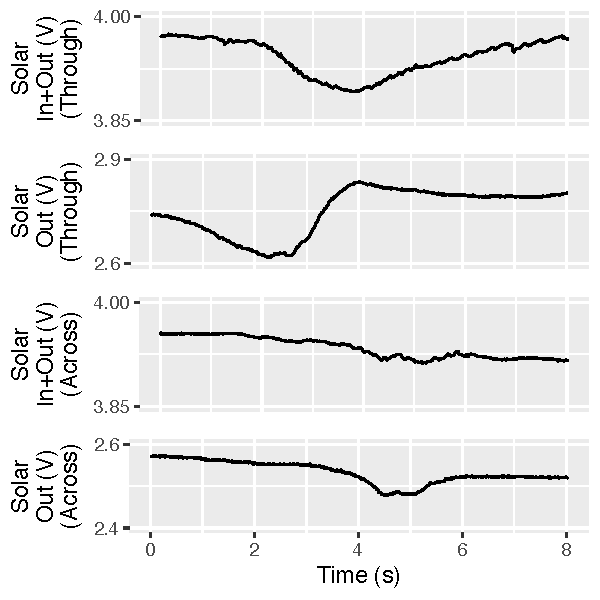
\includegraphics[width=\columnwidth]{figs/acrossAndLinger.pdf}
        \caption{ This figure provides a comparison between a person walking \textit{through} the doorway (top two traces) versus walking \textit{aross or by} the doorway on the outside. There is a clear delay between the two solar panel channels when someone walks through, whereas the change is reflected simultaneously when someone walks by.}
        \label{fig:across}
    \end{subfigure}
    \caption{Factors affecting \sysname operation. \label{fig:confounds}}
\end{figure*}


\subsubsection{Multiple people:}
\secref{sec:normal_operation} showed the ability of \sysname to detect individual people walking through.
A practical consideration would be to consider the performance of \sysname when multiple people walk through.

In order to evaluate this, we tested two subjects walking through doorway \#1 with varying time delay between them.
This gave us control over the time separation between two events, and allowed us to examine how closely can two people walk in without being detected as one, quite large person.
We discovered that as long as two people have at least \minSeparation between them, \sysname can accurately distinguish between them.
This limitation is introduced due to the time required by the solar panels to reset or stabilize before the next event can occur.
A subsequent logical conclusion is that if two people walk side-by-side, \ie with zero separation between them, the current setup of the system is unable to detect them as two events.

\subsubsection{The ``Spotlight'' effect:}
A very interesting consequence of light-based detection is what we affectionately call the \textit{spotlight effect}.
This effect appears in the presence of a very focused source of light that dominates the illumination around the doorway, such as a spotlight or a west-facing window in late evening when the sun blazes directly through.
When someone walks across such a focused light source, even if it's far from the doorway, it is detected falsely by \sysname as someone walking through.
This happens because \sysname detects people based on a decrease in the harvested energy, which also occurs when somenone momentarily blocks the focused source of light.
Interestingly, we can see from \figref{fig:spotlight} that the raw output of the solar panels look sufficiently different for someone walking \textit{across} the focused source as compared to when someone walks \textit{through} the doorway in presence of a focused source.
At present, \sysname is equipped to detect events with good accuracy.
With further signal processing, the difference between these events can be extracted so that such events will not cause false triggers.


\subsubsection{Detection Range/Walking across, not through:}
\label{subsubsec:range}
Considering that \sysname uses the blocking of light to detect a person, there will be an influence radius inside which a person starts affecting the harvested energy of the sensor.
If someone walks by either side of a doorway monitored by the \sysname sensor and are within the influence radius of the sensor, they will affect the sensor readings.
We ran an experiment to determine this radius of influence where the subject was directed to walk by on either side of the doorway at increasing distances from the sensor.
We started with a distance of 1 foot and went up to 5 feet, in increments of 1 foot.
For each distance, we asked the subject to walk by multiple times and recorded how many false triggers were detected.
Our findings are presented in \figref{fig:across}.
We have observed that for distances greater than 3 feet away from the doorway, there is a negligible chance of triggering false events.

It is interesting to note from \figref{fig:across} that there is a distinguishable difference between this event as compared to someone walking through the doorway.
Since they are walking only on one side of the doorway, their effect on both channels is not delayed by the angling of the solar panels, as is the case with walking through.
As with the ``Spotlight'' effect, we should be able to extract this difference with further signal processing and learning.

\subsubsection{Lingering in the doorway:}
Another situation that causes false triggers is when a person comes up to the doorway, but simply pokes their head in.
Upon evaluation, we discovered that as long as the person is poking their head in the doorway, the solar panel output remains at a lower level, and when they exit, it rises back again.
Although the current system implementation isn't equipped to differentiate between someone passing through and someone lingering in doorway, there is a clear difference in the raw waveform outputted by the solar panel.
This case is similar to \secref{subsubsec:range} in terms of being distinguishable from a person walking through and with some careful, direct signal processing it is definitely possible to differentiate between the actual and the confounding case.

\subsection{Microbenchmarks}
\label{sec:microbenchmarks}
The more effective \sysname is at maintaining a low-power state when idling, the more available \sysname is for detecting doorway events and monitoring occupancy.
The energy requirements for detection and active computation must be kept low as well.
Unlike intermittent computing sytems, \sysname must intentionally avoid power failures.
We measured the current draw of our \sysname prototype while it was mounted on doorway \#1.
The idle draw of the system was \SI{18}{\micro\ampere}, showing that \sysname can survive in a doorway with minimal light and energy harvesting.
We gathered other benchmarks of system energy performance in each mode of operation \sysname enters; the results of our experiments are shown in \tabref{tab:microbenchmarks}. These measurements were made after the MIC841 hysteresis chip, so the actual power and energy is slightly higher (by \SI{1.5}{\micro\ampere} according to the datasheet).


% Idle Current: 7-11uA, MCU not active
% Timer / ISR handling, single detector, no event : 190-230us, MCU active
% Doorway Event, MCU active, compute time: 7.2ms
%
% Peak current for active: 500uA
% Avg current for active: 220uA
% 2.8V
\begin{table*}[t]
\footnotesize
\caption{Microbenchmarks for \sysname energy consumption.}
\label{tab:microbenchmarks}
\begin{tabular}{@{}p{1.4in}lllc@{}}
\toprule
\textbf{State}          & \multicolumn{1}{r}{\textbf{Avg. Power}} & \multicolumn{1}{r}{\textbf{Peak Power}} & \multicolumn{1}{r}{\textbf{Energy Cost}} & \multicolumn{1}{r}{\textbf{MCU Active}} \\ \midrule
\textit{Waiting (Deep sleep)}       	& \SI{7}{\micro\ampere}	&  \SI{11}{\micro\ampere}	& - & \textcolor{magenta}{\xmark} \\
\textit{Maintenance Actions} & \SI{220}{\micro\ampere}	& \SI{500}{\micro\ampere}	& \SI{140}{\nano\joule}	 & \textcolor{green}{\cmark} \\
\textit{Doorway Event Handler} & \SI{220}{\micro\ampere}	& \SI{500}{\micro\ampere}	&  \SI{4424}{\nano\joule}     & \textcolor{green}{\cmark} \\ \midrule
\end{tabular}
\end{table*}


\tabref{tab:microbenchmarks} shows a low quiescent current where the MCU is asleep (the Idle state) of \SI{7}{\micro\ampere} on average. Maintenance events (from timer firing or single detectors firing from noise or people passing by the doorway but not walking through) only require \SI{140}{\nano\joule} to handle in active mode with the MCU running.
The most expensive compute operation is when the detectors fire and the MCU must compute the direction and store the results to non-volatile memory: FRAM. This costs \SI{4424}{\nano\joule}.
Overall the energy consumption of the system is low, but could be further improved with careful tuning of resistance values, sleep states, and the analog circuitry.

%\fxnote{[ I created  confusion matrix using R based on the collected data, but that data needs some cleaning like i+o, (i+)o in the %detected direction-AA]}
%section:  System Accuracy
	%just walking through
		%-just using interrupts
		%-just detection circuits
		%hw detection only vs sw enhancements
	%detecting direction
		%-just using interrupts
		%-just detection circuits
		%hw detection only vs sw enhancements
%if we get to sw at all





%section:  extreme cases (how low can we make lighting and system still work)?
